\documentclass[a4paper,12pt]{article}
\usepackage[hmargin=2cm,top=4cm,headheight=65pt,footskip=45pt]{geometry}
\usepackage[utf8]{inputenc}
\usepackage{graphicx}
\usepackage[hidelinks]{hyperref}
\usepackage{array}
\usepackage{lastpage}
\usepackage{lipsum}
\usepackage{fancyvrb}
\usepackage{color}
\usepackage{fancyhdr}
\usepackage{amsmath}
\usepackage{enumitem}
\usepackage{titlesec}
\usepackage{floatrow}
\usepackage{float}
\usepackage{subcaption}
\usepackage{caption}
\newfloatcommand{capbtabbox}{table}[][\FBwidth]

% Graphics path
\graphicspath{{figs/}}

\definecolor{customGray}{RGB}{128,128,128}
%\definecolor{Eblue}{RGB}{0,21,87}
%\definecolor{Eblue}{rgb}{0.2, 0.2, 0.6}
\definecolor{Eblue}{rgb}{0.0, 0.18, 0.39}
%==============Header & Footnote==============

\pagestyle{fancy}
\renewcommand{\headrulewidth}{0pt}
\fancyhead[C,CO,L,LO,R,RO]{}
\fancyhead[C]{%
          \begin{tabular}{|m{3.0cm}|m{10.0cm}|m{2.5cm}|}
          \hline
          \centering\vspace{1.75mm}
\includegraphics[scale=0.275]{logo.pdf} &
          \centering
          {\footnotesize {\sf UNIVERSIDAD EAFIT\\ SCHOOL OF ENGINEERING\\
          \vspace{-1mm}DEPARTMENT OF SYSTEMS AND INFORMATICS}} &
          \centering
          \footnotesize{Page \thepage\ de \pageref{LastPage}\\
          ST245\\
          \vspace{-0.75mm}Data Structures
          }\tabularnewline
          \hline
          \end{tabular}
}
\fancyfoot[C,CO,L,LO,R,RO]{}
\fancyfoot[C]{
          \begin{centering}
            \textcolor{customGray}{{\footnotesize {\sf Professor Mauricio Toro Bermúdez\\
            Phone: $(+57) (4) 261 95 00$ Ext. $9473$. Office: $19 - 627$\\
            \vspace{-1mm}E-mail: mtorobe@eafit.edu.co}}}
        \end{centering}
}

%=============CustomEnumItem===========

\setlist[enumerate]{label=\color{Eblue}\textbf{\roman*.}}

%=============CustomSecSubSec==========

\titleformat{\section}[hang]
{\normalsize\bfseries\itshape\color{black}}{\bfseries\itshape\color{Eblue}\thesection)}{2.5mm}{}

\titleformat{\subsection}[hang]
{\normalsize\bfseries\itshape\color{black}}{\bfseries\color{Eblue}\thesection.\alph{subsection}.}{2.5mm}{}


%==============Title==============

\title{\color{Eblue}\textbf{Laboratory practice No. 2: Big O Notation}}
\author{
  \textbf{Juan S. Cárdenas Rodríguez}\\
  Universidad EAFIT\\
  Medellín, Colombia\\
  jscardenar@eafit.edu.co
\and
  \textbf{David Plazas Escudero}\\
  Universidad EAFIT\\
  Medellín, Colombia\\
  dplazas@eafit.edu.co
}

%=============Document=============
\begin{document}
  \maketitle
  \thispagestyle{fancy}

  \section{CODE FOF \texttt{ARRAYSUM, ARRAYMAX, INSERTIONSORT, MERGESORT} WITH RANDOM ARRAYS}
    The \texttt{.py} file can be found in the ``codigo'' folder.
  \section{ONLINE EXERCISES (\texttt{CODINGBAT)}}
    The source code for all 10 exercises can be found in a \texttt{.java} file in ``ejercicioenlinea'' folder.
  \section{SIMULATION OF PROJECT PRESENTATION QUESTIONS}
    \subsection{Time for algorithms}
    \begin{table}[H]
      \centering
      \caption{Execution time for algorithms in nanoseconds.}
      \label{my-label}
      \begin{tabular}{ccccc}
        \hline
        \textbf{Input/Time(ns)} & \textbf{10} & \textbf{100} & \textbf{1000} & \textbf{100000} \\ \hline
        \textbf{ArrayMax}       & 5000        & 25000        & 450000        & 6250000         \\
        \textbf{ArraySum}       & 6000        & 22000        & 348000        & 6410000         \\
        \textbf{MergeSort}      & 31000       & 291000       & 3734000       & 45673000        \\
        \textbf{InsertionSort}  & 10000       & 445000       & 47573000      & 4655923000      \\ \hline
      \end{tabular}
    \end{table}

    \subsection{Plots for execution time}
    \begin{figure}[H]
        \begin{subfigure}[t]{0.49\textwidth}
            \centering
            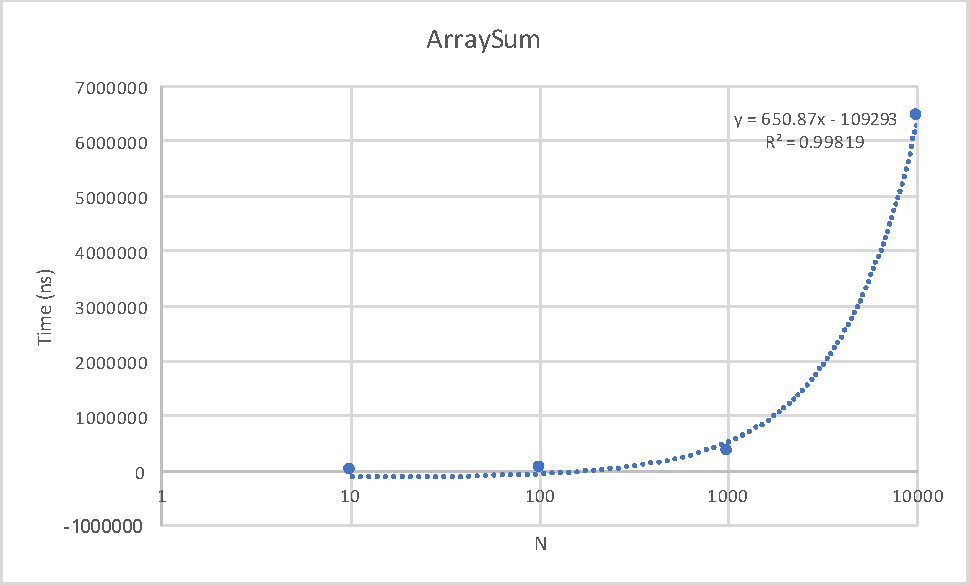
\includegraphics[width=\textwidth]{ArraySum.pdf}
            \caption{Time vs N for ArraySum}
        \end{subfigure}
        \begin{subfigure}[t]{0.49\textwidth}
            \centering
            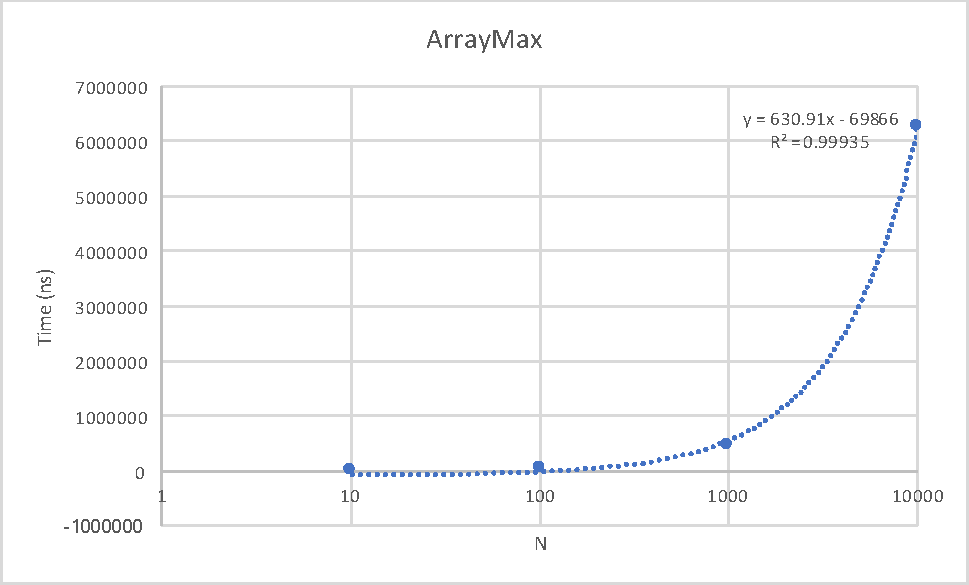
\includegraphics[width=\textwidth]{ArrayMax.pdf}
            \caption{Time vs N for ArrayMax}
        \end{subfigure}
        \caption{Array algorithms}
    \end{figure}

    \begin{figure}[H]
        \begin{subfigure}[t]{0.495\textwidth}
            \centering
            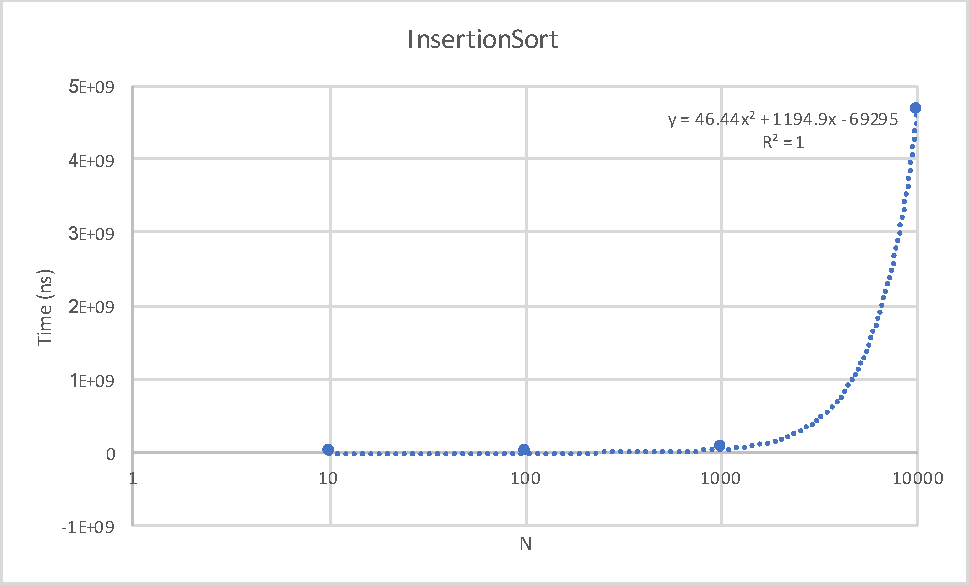
\includegraphics[width=\textwidth]{InsertionSort.pdf}
            \caption{Time vs N for InsertionSort}
        \end{subfigure}
        \begin{subfigure}[t]{0.495\textwidth}
            \centering
            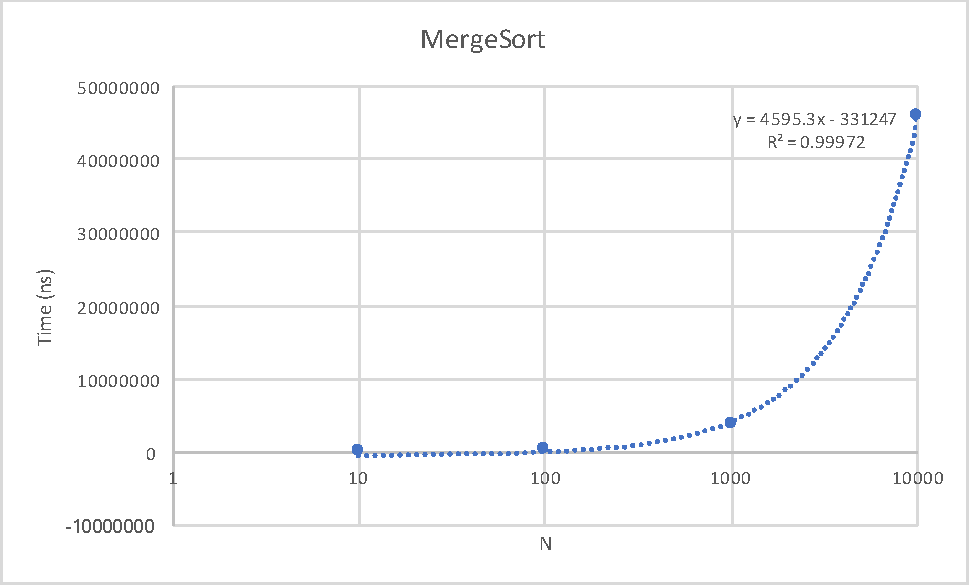
\includegraphics[width=\textwidth]{MergeSort.pdf}
            \caption{Time vs N for MergeSort}
        \end{subfigure}
        \caption{Sort algorithms}
    \end{figure}

    \subsection{What can you say between the results obtained and the theoretical \textit{Big-O} results?}
      According to the plots and the value of R, we can say that all of the algorithms execute within the interval of expected results;
      this is because all the results for R are really close to 1 (even one of them is exactly one), which allow us to affirm that the curve
      does indeed fit the data.

    \subsection{What happens to \texttt{insertionSort} for large N?}
      As we see in the graphics and the values, insertion sort has a asymptotical
      complexity of $n^2$. In this manner, we can see that if we use insertion sort for
      big numbers it will take a enourmous amount of time, so it will not be
      efficient in any shape or form.

  \subsection{What happens to \texttt{arraySum} for large N? Why does \texttt{insertionSort} increase faster?}
    As we know, the \textit{Big-O} notation tells us how does the function behave for large values of N.
    \texttt{arraySum} only makes one simple recursive call, thus \texttt{arraySum} is $O(n)$. This tells us
    that the execution time for \texttt{arraySum} increases linearly, proportional to the value of N. On the other hand,
    \texttt{insertionSort} is $O(n^2)$, which makes \texttt{arraySum} n times more efficent for the worst-case scenario.

  \subsection{How efficient is \texttt{mergeSort} with respect to \texttt{insertionSort} for large arrays?}
    The asymptotic complexity of \texttt{insertionSort} is $O(n^2)$, whereas for \texttt{mergeSort} is $O(n\log(n))$; it can be proved
    that $n\log(n)<n^2, \forall n\geq0$, therefore, \texttt{mergeSort} is more efficent than \texttt{insertionSort}.

  \subsection{How does \texttt{maxSpan} work?}
  \begin{Verbatim}
    def maxSpan(array):
      arr = []
      max = 0
      for i in range(len(array)):
        for j in range(i,len(array)):
          if array[i] == array[j]:
            c = j-i+1
        arr.append(c)
      for i in range(len(arr)):
        if arr[i] > max:
        max = arr[i]
      return max
  \end{Verbatim}
It works fairly easy. First for every data in the array of integers it moves
through the same array to the same index through the end of the array
searching for the number again. If it finds it again it sets the variable ``c''
to the numbers it has between them; it does this until the array ends. Then,
it searches the array to find the biggest span and returns that number.

\subsection{Array II}
  \begin{enumerate}
    \item \begin{Verbatim}
      public int[] zeroFront(int[] nums) {             // c0
          boolean [] used = new boolean [nums.length]; // c1
          int cont = 0;                                // c2
          for (int i = 0; i < nums.length; i++) {      // c3*n
            if(nums[i] == 0) {                         // c4*n
              if (i != cont) {                         // c5*n
                nums[i] = nums[cont];                  // c6+n
                nums[cont] = 0;                        // c7*n
              }
              cont++;                                  // c8*n
            }
          }
          return nums;                                 // c9
        }
    \end{Verbatim}
    Therefore, \texttt{zeroFront} is $O(c_0+c_1+c_2+c_9+(c_3+c_4+c_5+c_6+c_7+c_8)n)$,
    where n is the length of \texttt{nums}. Applying the sum and product properties,
    \texttt{zeroFont} is $O(n)$.

    \item \begin{Verbatim}
    public int[] notAlone(int[] nums, int val) {       // c0
        for(int i = 1; i < nums.length-1; i++) {       // c1*n
          if(nums[i] == val && nums[i-1] != val
            && nums[i+1] != val) {                     // c2*n
            if (nums[i-1] > nums[i+1])                 // c3*n
              nums[i] = nums[i-1];                     // c4*n
            else                                       // c5*n
              nums[i] = nums[i+1];                     // c6*n
          }
        }
        return nums;                                   // c7
      }
  \end{Verbatim}
  Therefore, \texttt{notAlone} is $O(c_0+c_7+(c_1+c_2+c_3+c_4+c_5+c_6)n)$, where n is the length of \texttt{nums}.
  Applying the sum and product properties, \texttt{notAlone} is $O(n)$.

  \item \begin{Verbatim}
  public boolean tripleUp(int[] nums) {                // c0
    for (int i = 0; i < nums.length - 2; i++) {        // c1*(n-2)
      if(nums[i] + 1 == nums[i+1] && nums[i]
       + 2 == nums[i+2]) return true;                  // c2*(n-2)
    }
    return false;                                      // c3
  }
  \end{Verbatim}
  \texttt{tripleUp} is $O(c_0+c_3+(c_1+c_2)(n-2))$, where n is the size of \texttt{nums}. When we apply the product
  and sum properties, \texttt{tripleUp} is $O(n)$.

  \item \begin{Verbatim}
  public int[] tenRun(int[] nums) {                   // c0
    int tempMult = 0;                                 // c1
    boolean used = false;                             // c2
    for(int i = 0; i < nums.length; i++) {            // c3*n
      if (nums[i] % 10 == 0) {                        // c4*n
        used = true;                                  // c5*n
        tempMult = nums[i];                           // c6*n
      }
      if(used)                                        // c7*n
        nums[i] = tempMult;                           // c8*n
    }
    return nums;                                      // c9
  }
  \end{Verbatim}
  \texttt{tenRun} is $O(c_0+c_1+c_2+c_9+(c_3+c_4+c_5+c_6+c_7+c_8)n)$, where n is the length of \texttt{nums}. When we apply
  the product and sum properties of the \textit{big-O} notation, yields that
  \texttt{tenRun} is $O(n)$.

  \item \begin{Verbatim}
  public int[] shiftLeft(int[] nums) {                // c0
    int [] mod = new int[nums.length];                // c1
    if (nums.length==1) return nums;                  // c2
    for (int i=1; i<nums.length; i++) {               // c3*n
      mod[nums.length-1]=nums[0];                     // c4*n
      mod[i-1]=nums[i];                               // c5*n
    }
    return mod;                                       // c6
  }
  \end{Verbatim}
  \texttt{shiftleft} is $O(c_0+c_1+c_2+c_6+(c_3+c_4+c_5)n)$, where n is the size of \texttt{nums}; which implies
  that \texttt{shiftLeft} is $O(n)$.
  \end{enumerate}

  \subsection{Array III}
  \begin{enumerate}
    \item \begin{Verbatim}
    public int[] seriesUp(int n) {                    // c0
      int no = n*(n+1)/2;                             // c2
      int [] nums = new int [no];                     // c3
      int a = 0;                                      // c4
      for (int i = 1; i <= n; i++) {                  // c5*n
        for (int j = 1; j <= i; j++) {                // c6*n*n
          nums[a] = j;                                // c7*n*n
          a++;                                        // c8*n*n
        }
      }
      return nums;                                    // c9
    }
    \end{Verbatim}
    \texttt{seriesUp} is $O(c_0+c_1+c_2+c_3+c_4+c_9+c_5n+(c_6+c_7+c_8)n^2)$,
    then \texttt{seriesUp} is $O(n^2)$.

    \item\begin{Verbatim}
    public int countClumps(int[] nums) {              // c0
      int c = 0;                                      // c1
      for (int i = 0; i < nums.length-1; i++) {       // c2*n
        if (nums[i] == nums[i+1]) {                   // c3*n
          for (int j = i; j < nums.length; j++) {     // c4*n*n
            if (nums[j] != nums[i]) {                 // c5*n*n
              i = j;                                  // c6*n*n
              c++;                                    // c7*n*n
            }
            if (c == 0 && j == nums.length-1) {       // c8*n*n
              c++;                                    // c9*n*n
            }
          }
        }
      }
      return c;                                       // c10
    }
    \end{Verbatim}
    \texttt{countClumps} is $O(c_0+c_1+c_10+(c2+c_3)n+(c_4+c_5+c_6+c_7+c_8+c_9)n^2)$, where n is the length of \texttt{nums};
    then \texttt{countClumps} is $O(n^2)$.
    \item \begin{Verbatim}

    public boolean linearIn(int[] outer,
      int[] inner) {                                  // c1
      int j = 0;                                      // c2
      int c = 0;                                      // c3
      if (inner.length == 0) return true;             // c4
      for (int i = 0; i < outer.length; i++) {        // c5*n
        if (inner[j] == outer[i]) {                   // c6*n
          j++;                                        // c7*n
          if (j==inner.length) {                      // c8*n
            return true;                              // c9*n
          }
        }
      }
      return false;                                   // c10
    }
    \end{Verbatim}
    \texttt{linearIn} is $O(c_1+c_2+c_3+c_4+c_10+(c_5+c_6+c_7+c_8+c_9)n)$, where n is the size of \texttt{outer};
    this implies that \texttt{linearIn} is $O(n)$.

    \item \begin{Verbatim}
    public int[] fix45(int[] nums) {                  // c1
      boolean [] arr = new boolean[nums.length];      // c2
      for (int i = 0; i < nums.length-1; i++) {       // c3*n
        if (nums[i] == 4 && nums[i+1] == 5) {         // c4*n
          arr[i+1] = true;                            // c5*n
        } else  if (nums[i] == 4 && nums[i+1] != 5) { // c6*n
          for (int j = 0; j < nums.length; j++) {     // c7*n*n
            if (nums[j] == 5 && arr[j] == false) {    // c8*n*n
              nums[j] = nums[i+1];                    // c9*n*n
              nums[i+1] = 5;                          // c10*n*n
              arr[i+1] = true;                        // c11*n*n
              break;                                  // c12*n*n
            }
          }
        }
      }
      return nums;                                    // c13
    }
    \end{Verbatim}
    \texttt{fix45} is $O(c_1+c_2+c_13+(c_3+c_4+c_5+c_6)n+(c_7+c_8+c_9+c_10+c_11+c_12)n^2)$, where n represents the length of \texttt{nums};
    this implies that \texttt{fix45} is $O(n^2)$.
    \item \begin{Verbatim}
    public boolean canBalance(int[] nums) {           // c0
      int sumRight;                                   // c1
      int sumLeft;                                    // c2
      for (int i = 1; i < nums.length; i++) {         // c3*n
        sumLeft = 0;                                  // c4*n
        sumRight = 0;                                 // c5*n
        for (int j = 0; j < i; j++) {                 // c6*n*n
          sumLeft += nums[j];                         // c7*n*n
        }
        for (int j = i; j < nums.length; j++) {       // c8*n*n
          sumRight += nums[j];                        // c9*n*n
        }
        if (sumRight == sumLeft) {                    // c10*n
          return true;                                // c11*n
        }
      }
      return false;                                   // c12
    }
    \end{Verbatim}
    \texttt{canBalance} is $O(c_0+c_1+c_2+(c_3+c_4+c_5+c_10+c_11)n+(c_6+c_7+c_8+c_9)n^2)$, where n is the size of \texttt{nums};
    therefore \texttt{canBalance} is $O(n^2)$.
  \end{enumerate}

  \section{EXAM SIMULATION}
  \begin{enumerate}
    \item c) $O(n+m)$
    \item d) $O(n*m)$
    \item b) $O(ancho)$
    \item b) $O(n^3)$
    \item d) $O(n^2)$
  \end{enumerate}


    %\newpage
    %\bibliographystyle{plain}
    %\bibliography{Lab.bib}
\end{document}
